%!TEX root = /Users/rafaeldurelli/Dropbox/Artigos Elaborados/KDM propagation_2015/sbes_2015_kdm_propagation/sbes2015_kdm_propagation.tex

A case study showing that our approach can be used to support the change propagation in KDM models is presented in this section. Throughout this case study we have used the described running example, i.e., we applied our three step approach in LabSys.
The object of this study is our proposed approach to propagate changes, and the purpose of this study is to evaluate the effectiveness of it. Taking into account the object and purpose of the study, we defined one research question:
\textit{ \textbf{RQ$_{caseStudy}$}: Given a set of refactoring (\textit{Extract Class}, \textit{Move Class}, \textit{Extract Layer} and \textit{Remove Class}),
can the proposed approach propagate all the changes effectively throughout KDM views}?


To assess the effectiveness of the proposed approach through the \textbf{RQ$_{caseStudy}$}, we use some oracles. As each refactoring has its own characteristics and modifies specific KDM model elements, it is possible to predict all the expected changes in other KDM views. So, considering our set of developed refactorings, we had to develop some oracles for each refactoring. The complete oracle can be seen at www.mudar.com.br.

The execution of this case study was assisted by our Eclipse plug-in that we developed to support the proposed approach. As stated in Section~\ref{sec:the_approach} the proposed approach uses as input two KDM instance, one representing the LabSys, and one conforming the refactored LabSys. Therefore, firstly we adopted a reverse engineering to transform the LabSys source-code into a KDM instance. We used MoDisco\cite{Brunele20141012}, which is a framework that get as input java source-code and then return as output a KDM instance. Currently, MoDisco only generates the KDM \texttt{Code package}, other KDM packages are extremely important to evaluate our approach. Therefore, we manually instantiated the followings KDM packages: \texttt{Structure Package}, \texttt{Data Package}, and \texttt{Conceptual Package}. After applying LabSys to MoDisco we gathered a KDM instance that contains 29,444 number of model instances (in this context KDM meta-classes' instances in the model). %The memory used on hard drive disk after XMI serialization is 5.66 MB. 

After that, we applied each refactoring and generated another KDM instances, i.e, this new KDM instance represent a new LabSys version, the refactored one. Then, we applied the step [B] of our approach - then a diff between the original KDM instance and the refactored one was performed. Finally, we applied the step [C] in order to propagate all the changes throughout KDM views. These steps were executed four times, i.e, for each chosen KDM refactoring all these step was performed.

As stated earlier, LabSys contains some flaws. More specifically, one an evident problem in this system is the presence of the ClassUnits \texttt{Student} and \texttt{Instructor} in the VIEW package, these ClassUnits should be allocated in the MODEL package. Another problem is that the ClassUnits \texttt{Laboratory} is doing work should be done by two ClassUnits. Similarly, by inspecting the LabSys instance we could notice that there is a ClassUnit that is no longer used, it does not contains any relationship with another ClassUnit. Finally, the \texttt{MODEL} Layer should also be extracted as it also contains internals elements responsible to deal with database information. 

In order to solve these flaws we selected selected three class-level refactorings (\textit{Extract Class}, \textit{Move Class} and \textit{Remove Class}) and one layer-level. The class-level refactorings are the conventional and well known Fowler's~\cite{refactImpro} refactorings easily found on literature. The conceptual order of applying these refactorings are botton-up, i.e., from lower level elements to higher level ones. For example, when you move classes from one package to another, business rules representing those classes should also be moved to other scenarios.

The refactoring  layer-level was intend to investigate top-down propagations, so, we decided to apply the \textit{Extract Layer} refactoring. The goal of this refactoring is the extraction of responsibilities from one layer and the moving of them to a recently created one. In this case, the propagation is from top to down, because it is necessary to propagate changes to lower level elements, such as Packages and ClassUnits, for example. 

It is important to highlight that all these KDM refactoring were devised in ATL. However, due space limitation only the refactoring \textit{Move Class} is depicted and explained.

\begin{figure}[h]
	\centering
	% Requires \usepackage{graphicx}
	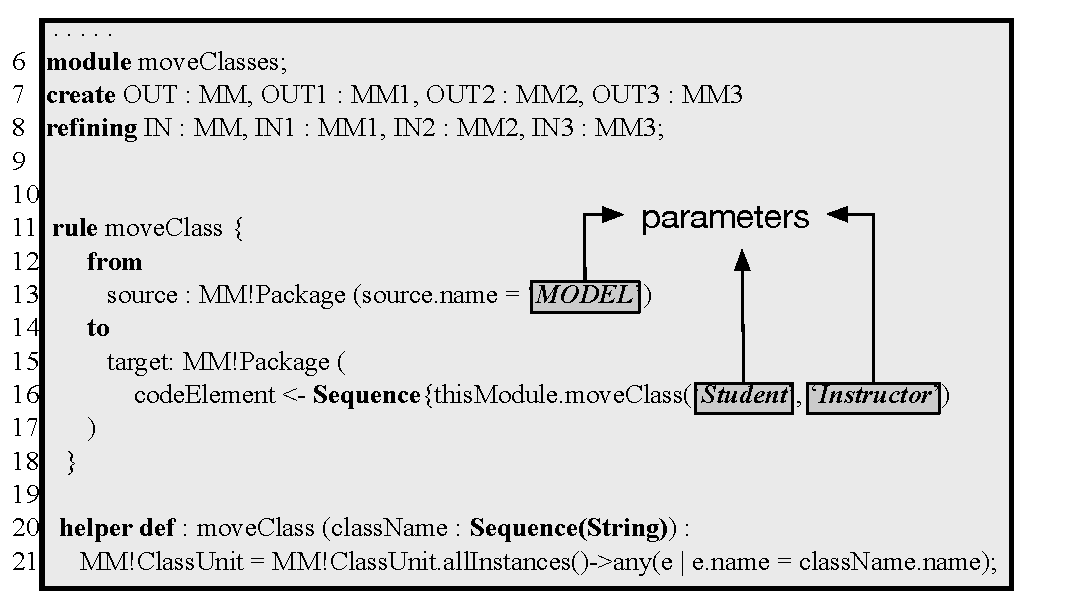
\includegraphics[scale=0.516]{figuras/NovoMoveClassFormatted}
	\caption{Snippet of ATL to perform the refactoring \textit{Move Class}.}
	\label{fig:ATLRefactoring}
\end{figure}

These KDM refactorings need parameters that should be informed before to start our three step approach. For instance, considering the refactoring illustrated in Figure~\ref{fig:ATLRefactoring} lines 13 and 16 three parameters specified, i.e, the source Package (\texttt{MODEL}) and two ClassUnit's instances (\texttt{Student} and \texttt{Instructor}) to be moved were specified. %that he(she) would like to move.
After specifying these parameters the ATL is ready to be applied into a KDM instance.


All refactorings were applied completely automatically by means of our devised plug-in, we just needed to specify all parameters. To deal with refactorings that go into infinite loops, we set three minutes timeout interval. 
%More specifically, 
We applied the \textit{Extract Class} to the ClassUnit \texttt{Laboratory}; we applied the \textit{Move Class} to two ClassUnit's instances (\texttt{Student} and \texttt{Instructor}); we applied the \textit{Extract Layer} to the \texttt{MODEL} Layer that contains internals elements to deal with database information; finally we applied the \textit{Remove Class} to a ClassUnit that was no longer used in LabSys.

The effect of applying these four KDM refactoring will turn the KDM instance inconsistent. For instance, considering the KDM refactoring \textit{Move Class} depicted in Figure~\ref{fig:ATLRefactoring} the ``density'' value will turn wrong, i.e., AggregationRelationShip between
the Layer VIEW and the Layer CONTROLLER would
change from 4 to 2 - once the primitives relationships Creates
and Extends would no longer exist from the package VIEW
to the package CONTROLLER. In the same way, the result of \textit{Move Class} refactoring should also update the density between the Layer
MODEL and CONTROLLER, instead of 2 it should be 4, as
Creates and Extends were also moved along with its
ClassUnits, \texttt{Student} and \texttt{Instructor}. Concerning to the
Conceptual View, the RuleUnit \textit{CheckFreeHours} that is associated with
\texttt{Instructor} should also be moved to ScenarioUnit \textit{RegisterStaff}. Others desynchronization would also arise after applying all described KDM refactorings. 

%moving these ClassUnits will turn the KDM instance inconsistent, because the ``density'' value will turn wrong, i.e., AggregationRelationShip between the Layer VIEW and the Layer CONTROLLER would change from 4 to 2 - once the primitives relationships Creates and Extends would no longer exist from the package VIEW to the package CONTROLLER. In the same way, the result of \textit{Move Class} refactoring should also update the density between the Layer MODEL and CONTROLLER, instead of 2 it should be 4, as Creates and Extends were also moved along with its ClassUnits, \texttt{Student} and \texttt{Instructor}. Concerning to the Conceptual View, the RuleUnit \textit{CheckFreeHours} that is associated with \texttt{Instructor} should also be moved to ScenarioUnit \textit{RegisterStaff}.
After applied all refactorings we verify whether them were successfully propagate throughout KDM views, i.e., if the intended refactoring could be performed and if all the expected propagations were generated on the KDM model. 
Based on a set of oracle it was possible to verify if all refactoring were successfully propagated throughout KDM models. Using these information gathered we can draw conclusion and answer the \textbf{RQ$_{caseStudy}$}. Table~\ref{tab:prop} summaries the results related to each refactoring applied and its respective propagations. In this table there are two abbreviations: (i) ``P.C?" (``Propagation Corrected?") and (ii) ``N.A" (``Not Applied"). This table also depicts the propagation regarding to the followings KDM packages: \texttt{Structure Package}, \texttt{Data Package}, and \texttt{Conceptual Package}. 

All the changes were effectively propagated throughout KDM views. Which means that in this case our approach could automatically execute truly relevant propagation in all KDM views when dealing with the chosen refactorings. Observing globally the data in Table~\ref{tab:prop} we can claim that the use of our approach in the context of these refactorings has been satisfactory. The data also show that our approach it is able to propagate changes in KDM view in an effective way and it also yields concise propagation of changes. Thereby, the \textbf{RQ$_{caseStudy}$} can be answered as true, that is, the proposed approach can propagate changes effectively throughout KDM views.

\begin{table*}
\centering
\caption{Propagations for the refactorings: Extract Class, Extract Layer, Move Class, and Remove Class\label{tab:prop}}
{\footnotesize{}}%
\setlength{\tabcolsep}{0.0em}
{\renewcommand{\arraystretch}{0.5}
\begin{tabular}{|l|>{\raggedright}p{7cm}|c|l|>{\raggedright}p{7cm}|c|}
\hline 
\textbf{\footnotesize{\cellcolor{gray!40}Refactoring}} & \textbf{\footnotesize{\cellcolor{gray!40}Extract Class}} & \textbf{\footnotesize{\cellcolor{gray!40}P.C?}} & \textbf{\footnotesize{\cellcolor{gray!40}Refactoring}} & \textbf{\footnotesize{\cellcolor{gray!40}Extract Layer}} & \textbf{\footnotesize{\cellcolor{gray!40}P.C?}}\tabularnewline
\hline 
\hline 
\multirow{4}{*}{{\footnotesize{Code}}} & {\footnotesize{Create an instance of ClassUnit that represent the
new Class}} & {\footnotesize{Yes}} & \multirow{2}{*}{{\footnotesize{Code}}} & {\footnotesize{Create an instance of Package}} & {\footnotesize{Yes}}\tabularnewline
\cline{2-3} \cline{5-6} 
 & {\footnotesize{Move all StorableUnits to the new ClassUnit}} & {\footnotesize{Yes}} &  & {\footnotesize{Move a set of selected ClassUnits from a Package to the
new Package}} & {\footnotesize{Yes}}\tabularnewline
\cline{2-6} 
 & {\footnotesize{Move all MethodUnit to the new ClassUnit}} & {\footnotesize{Yes}} & \multirow{4}{*}{{\footnotesize{Structure}}} & {\footnotesize{Create an instance of Layer}} & {\footnotesize{Yes}}\tabularnewline
\cline{2-3} \cline{5-6} 
 & {\footnotesize{Create an intance of HasType, which represent an association
between the new ClassUnit and the old ClassUnit}} & {\footnotesize{Yes}} &  & {\footnotesize{Create an instance of AggregationRelationship between
the new Layer and the old one}} & {\footnotesize{Yes}}\tabularnewline
\cline{1-3} \cline{5-6} 
{\footnotesize{Structure }} & {\footnotesize{N. A}} & {\footnotesize{N.A}} &  & {\footnotesize{Associate the new Layer by means of the association
implementation with the new Package}} & {\footnotesize{Yes}}\tabularnewline
\cline{1-3} \cline{5-6} 
\multirow{3}{*}{{\footnotesize{Data }}} & {\footnotesize{Create a instance of RelationalTable owning the name
of the new ClassUnit}} & {\footnotesize{Yes}} &  & {\footnotesize{Summing up all primitive relationship to compute the
meta-attribute density}} & {\footnotesize{Yes}}\tabularnewline
\cline{2-6} 
 & {\footnotesize{For each StorableUnit it is necessary to create a ItemUnit,
which represent the RelationaTable columns.}} & {\footnotesize{Yes}} & {\footnotesize{Data}} & {\footnotesize{N. A}} & {\footnotesize{N. A}}\tabularnewline
\cline{2-6} 
 & {\footnotesize{Create an instance of UniqueKey that represent the
primary key of the RelationalTable.}} & {\footnotesize{Yes}} & \multirow{2}{*}{{\footnotesize{Conceptual}}} & {\footnotesize{If the moved classes are associated to any conceptual
elements by means of the association implementation these conceptual
elements should be moved to a correspondent associated element of
the target Package.}} & \multirow{2}{*}{{\footnotesize{Yes}}}\tabularnewline
\cline{1-3} 
{\footnotesize{Conceptual}} & {\footnotesize{N. A}} & {\footnotesize{N. A}} &  &  & \tabularnewline
\hline 
\textbf{{\footnotesize{\cellcolor{gray!40}Refactoring}}} & {\textbf{\footnotesize{\cellcolor{gray!40}Move Class}}} & {\textbf{\footnotesize{\cellcolor{gray!40}P.C?}}} & {\textbf{\footnotesize{\cellcolor{gray!40}Refactoring}}} & {\textbf{\footnotesize{\cellcolor{gray!40}Remove Class}}} & {\textbf{\footnotesize{\cellcolor{gray!40}P.C?}}}\tabularnewline
\hline 
{\footnotesize{Code}} & {\footnotesize{Move an specific ClassUnti from a source Package to
a target Package}} & {\footnotesize{Yes}} & {\footnotesize{Code}} & {\footnotesize{Delete the selected instance of a ClassUnit}} & {\footnotesize{Yes}}\tabularnewline
\hline 
{\footnotesize{Structure}} & {\footnotesize{If the target Package is associated to an architectural
elements by means of the association implementation the value of meta-attribute
named density should be propagated}} & {\footnotesize{Yes}} & {\footnotesize{Structure}} & {\footnotesize{If the removed ClassUnit was contained into a specific
Structure element then summing up all primitive relationship and overwrite
the meta-attribute density}} & {\footnotesize{Yes}}\tabularnewline
\hline 
{\footnotesize{Data}} & {\footnotesize{N. A}} & {\footnotesize{N. A}} & {\footnotesize{Data}} & {\footnotesize{if the removed ClassUnit was associated with an instance
of RelationalTable, then it should also be removed}} & {\footnotesize{Yes}}\tabularnewline
\hline 
{\footnotesize{Conceptual}} & {\footnotesize{If the moved class is associated to any conceptual
elements by means of the association implementation this conceptual
elements should be moved to a correspondent associated element of
the target Package.}} & {\footnotesize{Yes}} & {\footnotesize{Conceptual}} & {\footnotesize{if the removed ClassUnit is associated to any conceptual
elements by means of the association implementation these conceptual
elements should be removed}} & {\footnotesize{Yes}}\tabularnewline
\hline 
\end{tabular}}
\end{table*}
